
\begin{figure*}[htbp]
    \begin{center}
        \centerline{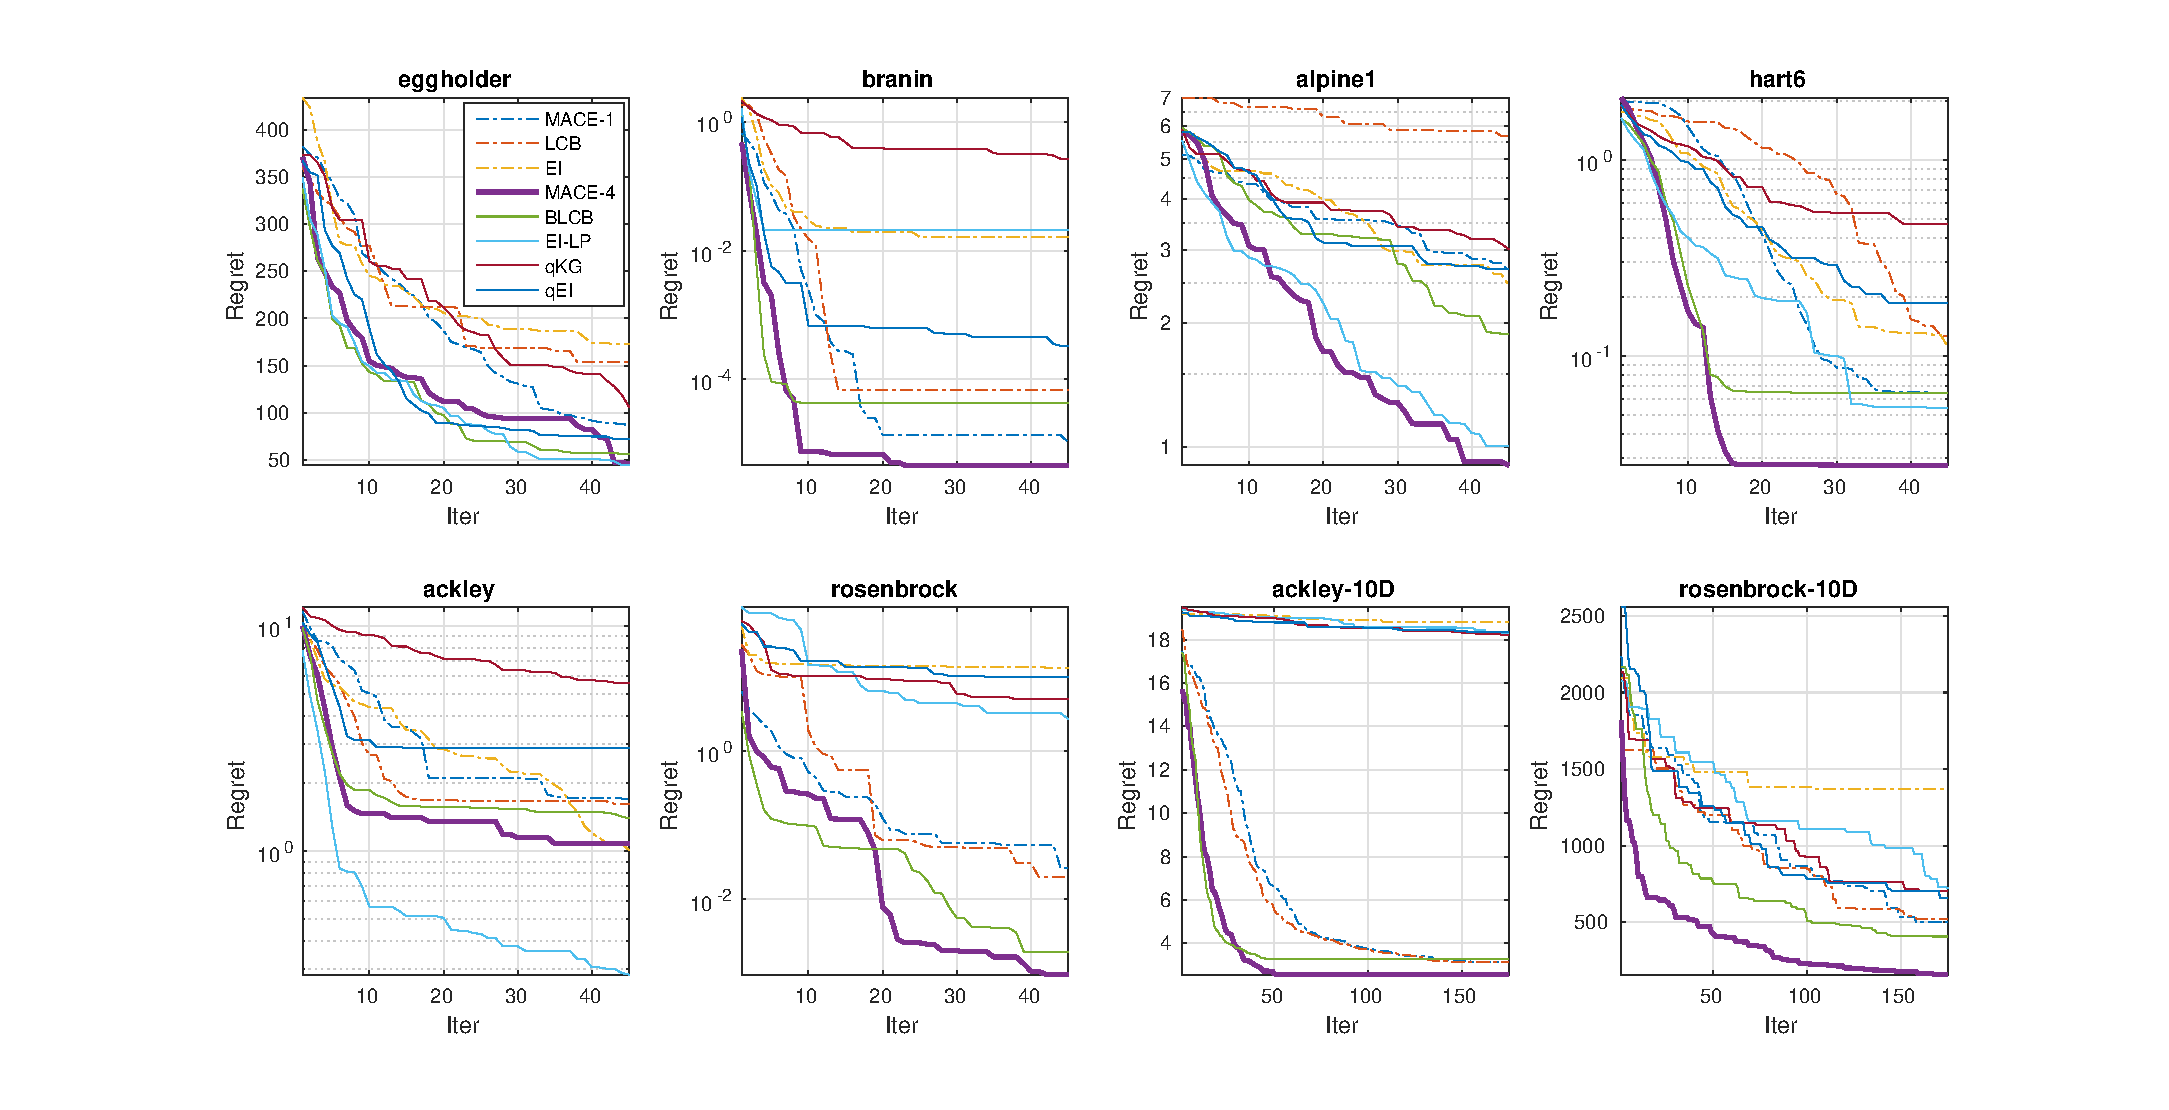
\includegraphics[width=1.0\linewidth]{./img/convplot.eps}}
        \caption{Optimization results of the benchmark functions}
        \label{fig:CovPlotBenchmark}
    \end{center}
\end{figure*}

\section{Experimental Results}

The proposed MACE algorithm was tested using eight benchmark functions and two
real-world circuits. Four state-of-the-art parallel Bayesian optimization
methods were compared, including the BLCB algorithm, the local penalization
method with EI acquisition function, the qEI and qKG methods\footnote{We
implemented the BLCB algorithm as the availble open source implementations only
allow discrete input; for the EI-LP method, the code is downloaded from
https://github.com/SheffieldML/GPyOpt is used; the code for qEI and qKG is
downloaded from https://github.com/wujian16/Cornell-MOE}.

\subsection{Benchmark Problems}

We tested the MACE algorithm and other parallel BO method using eight commonly used benchmark
functions, as summarized in Table~\ref{tab:summaryanalygical}.


\begin{table}[htbp]
    \centering
    \caption{Summary of the analytical benchmark functions}
    \label{tab:summaryanalygical}
    \begin{tabular}{llllllll}
        \toprule
         Function           & Dimension        & Search domain             \\ \midrule
         Branin             & 2                & $[-5,  10]\times[0, 15]$  \\
         Alpine1            & 5                & $[-10, 10]^5$             \\
         Hartmann6          & 6                & $[0,   1]^6$              \\
         Eggholder          & 2                & $[-512, 512]^2$           \\
         Ackley2            & 2                & $[-32, 32]^2$             \\
         Ackley10           & 10               & $[-32, 32]^{10}$          \\
         Rosenbrock2        & 2                & $[-5,  10]^2$             \\
         Rosenbrock10       & 10               & $[-20, 20]^{10}$          \\
        \bottomrule
    \end{tabular}
\end{table}

For all functions except the two 10D functions, we set the number of initial
random sampling to $N_{init} = 20$ and the number of iterations to $N_{iter} =
45$. Batch size is set to $B = 4$, the total number of function evaluations is
$N_{init} + B \times N_{iter}$. For the 10D Ackley and 10D Rosenbrock functions, we
$N_{init} = 100$ and $N_{iter} = 175$. The experiments were repeated ten
times to average the random fluctuations. 

We also ran the MACE algorithm in sequential mode and compared with the EI and LCB
acquisition functions, the sequential EI and LCB based Bayesian optimization
are implemented by setting the batch size $B = 1$ for EI-LP and BLCB
respectively.

The mean convergence plot is shown in Figure~\ref{fig:CovPlotBenchmark}. The
statistics of the final optimization results are listed in
Table~\ref{tab:result_analytical}. As can be seen, when running with batch size
$B = 4$, the MACE algorithm gives the best performance for six out of the eight
benchmarks.  For the 2D Ackley function, EI-LP is the best algorithm, while for
the Eggholder function, the MACE, BLCB, and EI-LP have quite similar
performance.  Compare the batch MACE and the sequential MACE, the speedup is
also dramatic.

% \begin{table*}[tp]
%     \tiny
%     \centering
%     \caption{Optimization results of the benchmark functions}
%     \label{tab:result_analytical}
%     \begin{tabular}{lllllllllll}
%         \toprule
%         Function    & MACE-1             & LCB-1                 &  EI-1                 &  MACE-4               & BLCB-4                &  EI-LP-4              & qKG-4                   & qEI-4                     \\ \midrule
%         Eggholder   & 88$\pm$76          &  1.5e+2$\pm$1.1e2     &  1.7e2$\pm$1.3e2      &  46$\pm$41            &  57$\pm$36            &  45$\pm$56            &  1.1e2$\pm$68  &  72$\pm$52            & \\
%         Branin      & 1e-5$\pm$1.3e-5    &  6.9e-5$\pm$1.1e-4    &  0.016$\pm$0.016      &  4.6e-6$\pm$6.6e-6    &  4.3e-5$\pm$6.3e-5    &  0.021$\pm$0.018      &  0.27$\pm$0.27 &  3.3e-4$\pm$1.1e-3    & \\
%         Alpine1     & 2.7$\pm$1.1        &  5.7$\pm$1.8          &  2.5$\pm$1.6          &  0.9$\pm$0.84         &  1.9$\pm$0.94         &  1$\pm$0.46           &  3$\pm$1.1     &  2.7$\pm$1.1          & \\
%         Hart6       & 0.065$\pm$0.062    &  0.13$\pm$0.12        &  0.11$\pm$0.15        &  0.028$\pm$0.052      &  0.064$\pm$0.062      &  0.054$\pm$0.056      &  0.47$\pm$0.19 &  0.19$\pm$0.12        & \\
%         Ackley      & 1.7$\pm$1.1        &  1.6$\pm$0.93         &  1$\pm$0.99           &  1.1$\pm$0.89         &  1.4$\pm$1            &  0.28$\pm$0.25        &  5.6$\pm$1.8   &  2.9$\pm$1            & \\
%         Rosenbrock  & 0.026$\pm$0.051    &  0.02$\pm$0.021       &  14$\pm$9.5           &  9.5e-4$\pm$9.4e-4    &  1.9e-3$\pm$1.8e-3    &  2.7$\pm$2.1          &  5$\pm$3.7     &  10$\pm$15            & \\
%         G05         & 3.1$\pm$0.45       &  3.1$\pm$0.52         &  19$\pm$0.65          &  2.6$\pm$0.54         &  3.3$\pm$0.74         &  18$\pm$0.61          &  18$\pm$0.76   &  18$\pm$0.5           & \\
%         G07         & 500$\pm$300        &  520$\pm$290          &  1400$\pm$640         &  160$\pm$50           &  410$\pm$130          &  720$\pm$330          &  710$\pm$410   &  660$\pm$340          & \\
%         \bottomrule
%     \end{tabular}
% \end{table*}


\begin{table*}[t]
    \centering
    \caption{Optimization results of the benchmark functions}
    \label{tab:result_analytical}
    \begin{tabular}{lllllllllll}
        \toprule
                    & MACE-1                & LCB-1                 &  EI-1                 &                & \\ \midrule
        Eggholder   & 88$\pm$76             &  1.5e+2$\pm$1.1e2     &  1.7e2$\pm$1.3e2      &                & \\
        Branin      & 1e-5$\pm$1.3e-5       &  6.9e-5$\pm$1.1e-4    &  0.016$\pm$0.016      &                & \\
        Alpine1     & 2.7$\pm$1.1           &  5.7$\pm$1.8          &  2.5$\pm$1.6          &                & \\
        Hart6       & 0.065$\pm$0.062       &  0.13$\pm$0.12        &  0.11$\pm$0.15        &                & \\
        Ackley      & 1.7$\pm$1.1           &  1.6$\pm$0.93         &  1$\pm$0.99           &                & \\
        Rosenbrock  & 0.026$\pm$0.051       &  0.02$\pm$0.021       &  14$\pm$9.5           &                & \\
        G05         & 3.1$\pm$0.45          &  3.1$\pm$0.52         &  19$\pm$0.65          &                & \\
        G07         & 500$\pm$300           &  520$\pm$290          &  1400$\pm$640         &                & \\
        \hline
                    &  MACE-4               & BLCB-4                &  EI-LP-4              & qKG-4          & qEI-4                 \\ \midrule
        Eggholder   &  46$\pm$41            &  57$\pm$36            &  45$\pm$56            &  1.1e2$\pm$68  &  72$\pm$52            \\
        Branin      &  4.6e-6$\pm$6.6e-6    &  4.3e-5$\pm$6.3e-5    &  0.021$\pm$0.018      &  0.27$\pm$0.27 &  3.3e-4$\pm$1.1e-3    \\
        Alpine1     &  0.9$\pm$0.84         &  1.9$\pm$0.94         &  1$\pm$0.46           &  3$\pm$1.1     &  2.7$\pm$1.1          \\
        Hart6       &  0.028$\pm$0.052      &  0.064$\pm$0.062      &  0.054$\pm$0.056      &  0.47$\pm$0.19 &  0.19$\pm$0.12        \\
        Ackley      &  1.1$\pm$0.89         &  1.4$\pm$1            &  0.28$\pm$0.25        &  5.6$\pm$1.8   &  2.9$\pm$1            \\
        Rosenbrock  &  9.5e-4$\pm$9.4e-4    &  1.9e-3$\pm$1.8e-3    &  2.7$\pm$2.1          &  5$\pm$3.7     &  10$\pm$15            \\
        G05         &  2.6$\pm$0.54         &  3.3$\pm$0.74         &  18$\pm$0.61          &  18$\pm$0.76   &  18$\pm$0.5           \\
        G07         &  160$\pm$50           &  410$\pm$130          &  720$\pm$330          &  710$\pm$410   &  660$\pm$340          \\
        \bottomrule
    \end{tabular}
\end{table*}

\subsection{Operational Amplifier}

%TODO: Introduce the importance of OpAmp and PA

\textcolor{red}{TODO: if possible, run qKG and qEI for this circuit}

The operational amplifier~\cite{wang2014enabling} shown in
Figure~\ref{fig:schDAC2014} is used for comparison, the circuit is designed
using the 180nm process. It has ten design parameters, including the lengths
and widths of transistors, the resistance of resistors and the capacitance of
capacitors. The circuit is simulated using the HSPICE circuit simulator.

We want to maximize the gain, unit gain frequency (UGF) and the phase margin (PM) for this amplifier, the $FOM$ is constructed as:
$$
\mathit{FOM} = -1.2 \times \mathit{gain} - 10 \times \mathit{UGF} - 1.6 \times \mathit{PM}
$$

For this circuit, we compared the MACE algorithm with the BLCB and EI-LP
algorithms, the qKG and qEI are not compared as the calculation of qEI and qKG
acquisition functions become very slow for the ten-dimensional functions. 


\begin{figure}[h]
    \begin{center}
        \centerline{\includegraphics[width=\columnwidth]{./img/sopam.pdf}}
        \caption{Schematic of the operational amplifier}
        \label{fig:schDAC2014}
    \end{center}
\end{figure}

\begin{figure}[]
\vskip 0.2in
\begin{center}
\centerline{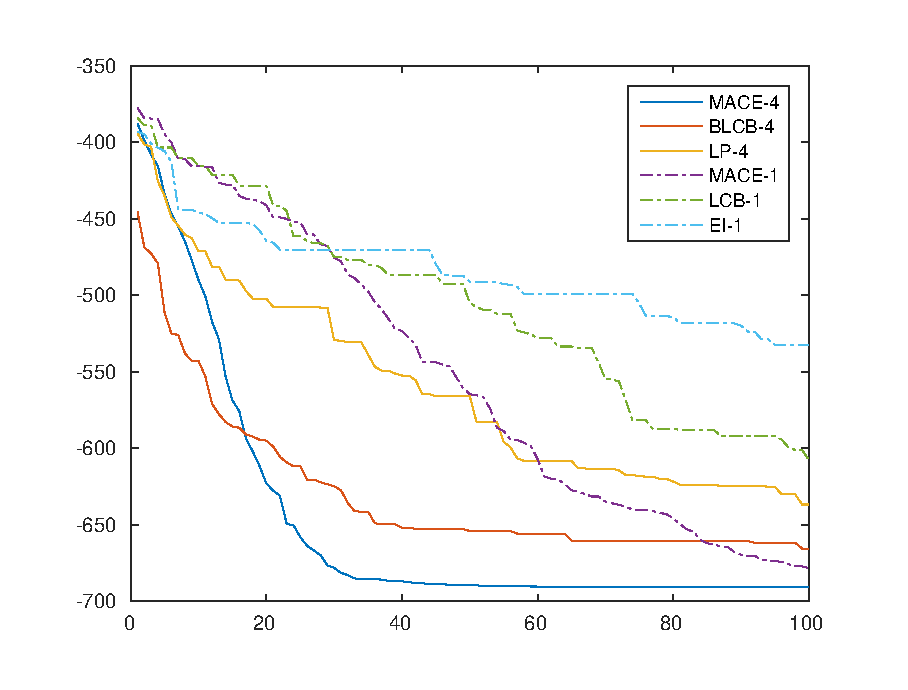
\includegraphics[width=\columnwidth]{./img/mean_DAC2014.eps}}
\caption{Optimization results of the operational amplifier}
\label{fig:resDAC2014}
\end{center}
\vskip -0.2in
\end{figure}

We run the algorithms in sequential mode and batch mode, for the batch
mode, batch size is set to $B = 4$. The number initial random sampling is set
to $N_{init} = 100$, and the number of iterations is set to $N_{iter} = 100$.


\begin{table}[h]
    \centering
    \caption{Optimization results of the operational amplifier}
    \label{tab:result_opamp}
    \begin{tabular}{llll}
        \toprule
        Algorithm & Results     \\ \midrule
        MACE-1    & 0.0$\pm$0.0 \\
        LCB-1     & 0.0$\pm$0.0 \\
        EI-1      & 0.0$\pm$0.0 \\
        MACE-4    & 0.0$\pm$0.0 \\
        BLCB-1    & 0.0$\pm$0.0 \\
        EI-LP-4   & 0.0$\pm$0.0 \\
        \bottomrule
    \end{tabular}
\end{table}

The mean convergence plot for the sequential and batch runs are plotted in
Figure~\ref{fig:resDAC2014}. As can be seen, the MACE algorithm gave better
solution compared with other algorithms, the sequential MACE algorithm found
better solution than BLCB and EI-LP with batch size $B = 4$, which showed that
the multi-objective acquisition ensemble is more robust than relying on single
acquisition function; compared with the sequential MACE algorithm, the MACE
algorithm with batch size $B = 4$ showed considerable speedup.


\subsection{Class-E Power Amplifier}


\begin{figure}[htbp]
    \begin{center}
        \centerline{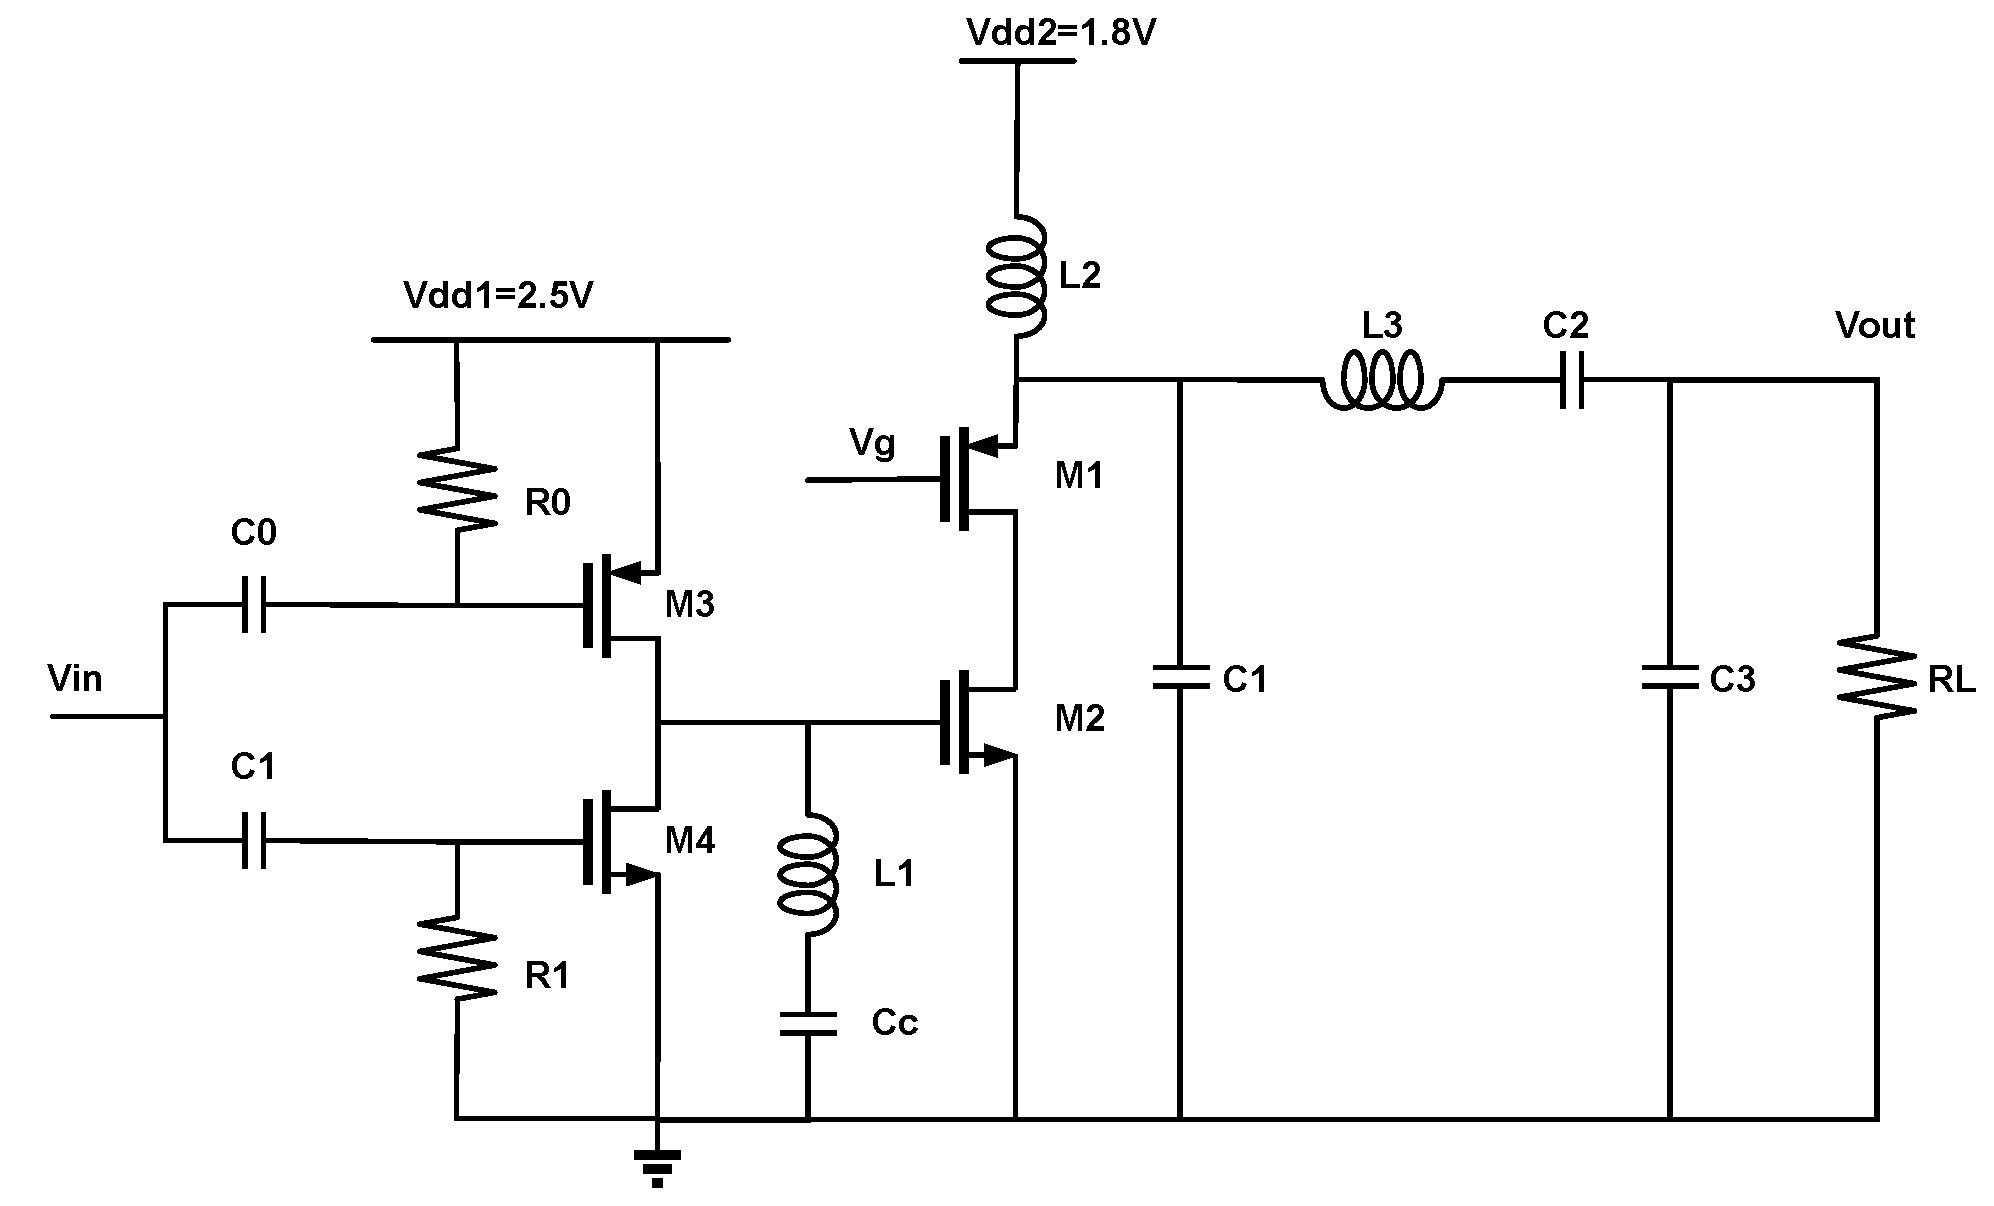
\includegraphics[width=\columnwidth]{./img/classE.eps}}
        \caption{Schematic of the power amplifier}
        \label{fig:schPA}
    \end{center}
\end{figure}

The power amplifier shown in Figure~\ref{fig:schPA} is used for comparison, the
circuit is designed using the 180nm process with twelve design parameters, the
circuit is simulated by HSPICE to get its performances.

For this power amplifier, we aim to maximize the power added efficiency (PAE) and the output power (Pout), the $FOM$ is constructed as
$$
\mathit{FOM} = -3 \times \mathit{PAE} - \mathit{Pout}
$$

\begin{table}[htbp]
    \centering
    \caption{Optimization results of the power amplifier}
    \label{tab:result_PA}
    \begin{tabular}{llll}
        \toprule
        Algorithm & Results     \\ \midrule
        MACE-1    & 0.0$\pm$0.0 \\
        LCB-1     & 0.0$\pm$0.0 \\
        EI-1      & 0.0$\pm$0.0 \\
        MACE-4    & 0.0$\pm$0.0 \\
        BLCB-1    & 0.0$\pm$0.0 \\
        EI-LP-4   & 0.0$\pm$0.0 \\
        \bottomrule
    \end{tabular}
\end{table}

The MACE, BLCB, and EI-LP algorithms were tested in both sequential and batch
mode. The number of initial sampling is $N_{init} = 100$, the number of
iterations is $N_{iter} = 100$, the batch size is set to $B = 4$, so the total
number of HSPICE simulations is 500 for each batch run and 200 for each
sequential run.


\begin{figure}[htbp]
\vskip 0.2in
\begin{center}
\centerline{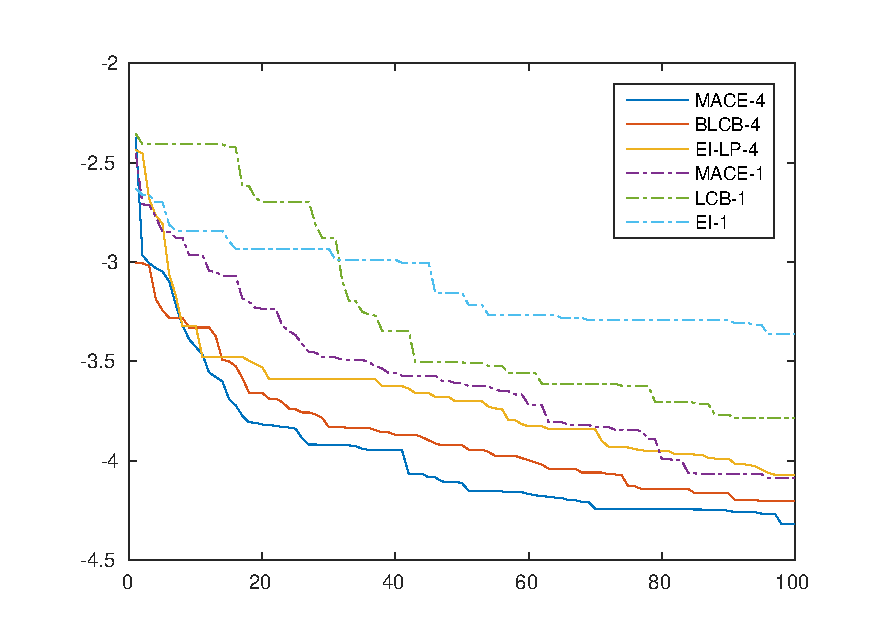
\includegraphics[width=\columnwidth]{./img/ClassE_mean.eps}}
\caption{Optimization results of the class-E power amplifier}
\label{fig:resClassE}
\end{center}
\vskip -0.2in
\end{figure}

The mean convergence plot is given in Figure~\ref{fig:resClassE}. We can see
that the MACE outperformed the BLCB and EI-LP in both sequential and batch
mode. For the batch runs, the MACE convergences fastest among the three
algorithms, while the sequential MACE has similar performance as the batch
EI-LP method.
